\chapter{CASE STUDIES}\label{CASE STUDIES}
This Section contains three case studies which illustrate the application of the VSM to co-operatives of different sizes.

The first involves a small co-operative of 5 people, and clarifies the mechanisms whereby a small unstructured group can demonstrate viability.

The second describes a study of a medium size group of 35 people who were experiencing organisational difficulties, the conclusions that were reached using the VSM, and what happened when they were put into practice.

The third involves the (huge) Mondragon co-operatives in an attempt to see if the VSM can throw any light on their astonishing success.

\section*{Case Study 1: HEBDEN WATER MILLING COLLECTIVE 1985}
I began with HWMC because at that time it was the enterprise that I knew most about.

I had been involved in setting it up in 1980, and had seen it grow and prosper in its first five years without any formal structure.

The task I had set myself was to see if the VSM could describe the mechanisms which enable a small loose co-operative to function in an undeniably viable fashion.

Or ... if the VSM had said "this just can't be viable as you don't have a System X, and that's a fundamental of all viable systems" ... I would have had serious doubts about its usefulness to co-operatives.

\section*{Background}
HWMC is a small co-operative that was formed in 1980 to blend and package a large range of wholefoods using fairly complicated machinery.

For the period 1980 - 1985, HWMC was successful both in its financial performance and in the working environment it provided for its members. The production processes became extremely efficient, crises were dealt with effectively, challenges were met and discharged, relations between the members were excellent, profits were good, and in general the system worked beautifully.

All decisions were made by consensus, and weekly meetings (when necessary) usually lasted about ten minutes.

Working procedures evolved during the day: after a 30 second planning session ("Let's do the Basmati rice first"), everyone would work around each other, without formal planning, and the days production would proceed. The process is much more in sympathy with the operation of a Jazz band or a football team: basic rules and constraints are understood, but the specific actions performed by the participants are dictated by the conditions of the moment.

\[As an aside, I should mention that working in this way has been one of the most satisfying experiences that I have had, and goes some way to explain why co-operatives are full of graduates doing apparently boring manual jobs.\]

\section*{Preliminary Diagnosis}
The initial diagnosis began with the five members positioned as the Operational units. The Metasystem was also composed of all five members, but in a different role: when the work was being done they were \textbf{Operation}, when planning was necessary they articulated the \textbf{Metasystem}. The fundamental co-operative principle of \textbf{self-management} means that there is no clear division in the roles of people working within the group: everyone is obliged to be both "manager" and "worker."

Generally, as the diagnosis proceeded it became obvious that as a function was identified (for example a System 2 stability function whereby the available worker-power was effectively allocated to the various tasks) the same principle was in operation: all members identified the need to articulate a particular Metasystemic function - often without verbal acknowledgement - and shifted into the appropriate mode to deal with the situation.

In many cases, the Metasystemic functions could be done while the Operational work was proceeding (we're nearly at the end of this run ... has anyone got the next one ready?) whereas other discussions required the temporary suspension of manual work, or in unusually complicated situations a few hours put aside to generate plans and strategies.

\section*{The Mechanics of Viability at HWMC}
\begin{itemize}
  \item Most Metasystemic activity (systems 2 and 3) is present continuously.

  \item Work proceeds as described above. As long as nothing unexpected occurs very little Metasystemic activity is needed. Most Metasystemic activity (systems 2 and 3) is present continuously.

  \item The \textbf{model of the Operation}, located in System 3 and crucial to viability, is continuously being upgraded in the minds of the members. Thus the System 3 model is up to date and virtually complete. (It even knows if someone changes his shirt.)

  \item \textbf{Instabilities} in the production techniques are usually dealt with immediately for two reasons: firstly, all members share a compatible System 3 model; and secondly, the performance of the Operational elements is based on co-operation and not competition.

\end{itemize}

.-   The Metasystem is alerted immediately it is needed: any crisis (for example a sudden large demand for muesli, or a machinery breakdown) suspends the Operational activity briefly and the Metasystem springs into action - that is everyone goes into a huddle; \["Can we cope?" "I can do a couple of hours after work." "Jack is free tomorrow lets get him in."\] and so on.

\begin{itemize}
  \item The operation of System 4 is firmly based on the System 3 model, and as long as long as everyone has their wits about them , the whole thing works very effectively.
\end{itemize}

\section*{Conditions for Viability in a Small Group}
Having experienced this process for a number of years, it is apparent that three conditions are necessary for viability. They are as follows:

\begin{enumerate}
  \item Everyone must be capable of, and involved in, both Operational and Metasystemic functions: if this is not the case, the capabilities of the Metasystem will not be sufficient to deal with the Operation.

  \item Efforts must be made to ensure the completeness and availability of the System 3 model. In HWMC, everyone was present most of the time, so there was no problem.

  \item The mechanics of viability are completely dependant on \textbf{thorough discussion}. Effective discussion is essential in the generation of the System 3 model, the workings of the necessary interaction between System 3 and System 4, and the successful discharge of all Metasystemic functions.

\end{enumerate}

Usually, in a group of four or five people, there is no problem in satisfying these three prerequisites, and viability is relatively straightforward provided that everyone works as a team for the majority of the time and the need for all the Metasystemic functions, especially future planning, is recognised.

There would seem to be nothing to prevent a non-structured organisation of this kind working Viably.

\section*{The Collapse of Viability in a Small Co-operative}
The weakness of the kind of structure exhibited by HWMC is that viability is entirely dependant on the people involved. There is no formal structure to ensure effective viability. Consequently it is not uncommon for the group to degenerate into a non-viable form.

\section*{1. Problems with the Metasystem}
There are many ways in which the capabilities of the Metasystem can be affected. For example, if a new member lacks confidence he may not feel able to enter into a Metasystemic function, as this may be seen to be the province of more experienced members. Thus vital information may not be forthcoming in a System 3 meeting.

Exactly the same problem may emerge if the "old hands", by their attitudes, discourage new members from becoming involved at all levels.

There also seems to be a potential danger that in a co-operative which involves much concentration at the Operational level (say a co-operative of computer programmers) very little brain power will be left to deal with Metasystemic issues. In this case it may be necessary to appoint a member to deal mainly with Metasystemic issues, and in this case a different organisational structure will be needed.

A further problem could emerge in a period of continuous crisis when the Metasystemic functions need such a large amount of the time that the Operational functions are neglected (that is, no production gets done). This could be overcome by extending production time, but again the division of the Operational and Metasystemic functions is a possible solution.

\section*{2. Problems with the System 3 Model}
One of the more common complaints from people who deal regularly with co-operatives is that essential information is not available when it's needed.

This may be caused by movement of members (the relevant information was given to Jill who is out driving today ...), by feelings of unimportance (Jack doesn't think he's valued enough to make a contribution, although he may know the crucial element ...), and so on.

Recognition of the absolute necessity of the System 3 model for viability may be one of the more important contributions of VSM theory to co-ops. It may also avoid the usual knee-jerk reaction to the lack of the System 3 model which is: appoint a manager. Although this would allow a complete System 3 model to be generated (the Manager would act as a reference point for everyone and would thus accumulate the necessary information), other ways may be more appropriate such as a computer model or a large blackboard or magnetic shapes on a sheet of metal.

\section*{Summary: Conditions for Viability}
A small group may demonstrate viability as long as:

\begin{enumerate}
  \item All members are capable of both Operational and Metasystemic functions
(i.e. they can do the basic work and discuss optimisation, policy, future plans ...)

  \item All members are present all the time. Metasystemic functions need to refer to a real-time complete model of the Operation. If some people are not present, and they have the crucial information needed for a decision, then that decision will be made in ignorance.

  \item All decisions must be based upon thorough discussion by all members.

  \item All Metasystemic functions must be recognised and performed.

  \item The need to keep an eye on the external environment must be recognised, and this information should be used to generate plans to adapt to the future.

\end{enumerate}

\section*{Conclusion}
Having worked in this kind of co-operative for many years and experienced just how efficient and rewarding it can be, it is clear from the VSM analysis that two conclusions may be made:

\begin{enumerate}
  \item This kind of unstructured small group is able to demonstrate viability in the terms used in VSM studies.

  \item This viability is fragile.

\end{enumerate}

The first three conditions for viability are not impossible to meet, but viability can collapse as membership changes, members' personalities clash, some people feel they can take on Metasystemic jobs without consultation, and so on. Condition 2 is obviously difficult due to holidays and sickness, and thus the Metasystem will occasionally have to cope with an incomplete model.

Two recommendations may be offered

\begin{itemize}
  \item That daily performance indicators are measured and displayed in meeting places. This will complement the model of the Operation which accumulates during work and discussions, and if viability does begin to collapse, there will be immediate alerting signals.

  \item That there are regular slots on the agenda to discuss internal optimisation and future plans to ensure these two conditions for viability are met.

\end{itemize}

\section*{Case Study 2: TRIANGLE WHOLEFOODS}
This Case Study examines the problems which had emerged at Triangle Wholefoods (trading as \href{http://www.suma.co.uk/}{Suma}) as it grew from a small group to become one of the largest co-operatives in the UK.

It is clear that as numbers grow, meetings become more and more difficult. There are various ways of looking at this but the basic principle is clear: small meetings work - large ones don't.

The exact numbers vary with the type of organisation but in general under 11 is easy, between 11 and 20 is difficult but manageable, above 20 is just unworkable without very small agendas, lots of preparation and rigid control from the chair.

Suma was attempting to perform all its management through a single weekly meeting of all members, and it clearly was not working.

The task of the VSM was to design an effective organisation without resorting to managers, or authority/obedience techniques.

\textbf{Note:}

The material in this section was written in 1986, with additional material added in 1991.

\section*{Background}
TRIANGLE WHOLEFOODS, trading as Suma, began in the mid seventies with a loan of £4,000 and was supported by the five wholefood retail co-operatives in the north of England who agreed to buy everything they could through Suma. This gave Suma a guaranteed minimum turnover.

Over the following three years, the number of wholefood co-operative shops in the region grew enormously to around 60 by 1980, and Suma prospered accordingly.
Since that time the co-operatives have become a less and less important part of Suma's turnover: there are now around 2,500 customers.

Currently (1998) Suma operates in a 60,000 sq. ft. warehouse in Halifax, offers a range of about 7,000 products (3,000 in 1991, 5,000 in 1995), and distributes nationally with a growing number of exports. There is some in-house pre-packing and bottling. Recent years have seen the introduction of several own-label products and the growth of environmentally sound products.

Suma has always attempted to base its working practices upon the needs of its members - job rotation and flexible working conditions are common. Equal numbers of men and women has generally been achieved.

At the time I was applying these ideas, SUMA, consisted of about 35 workers with a turnover in the region of 6 million ECU.

Some departments had evolved (transport, manufacturing, warehouse), there were two committees which considered financial and personnel matters, and the entire membership was supposed to meet for the weekly Management Meeting every Wednesday afternoon. This meeting was the \textbf{only} recognised decision making body within Suma, and as such had to deal with all departmental issues as well as Suma policy. It also had to ratify the recommendations from the committees.

The problem which had triggered the VSM study was an almost universal recognition that the Wednesday meetings were not working. As the size increased, agendas were getting longer and longer, less and less was getting dealt with, arguments were common, and many people didn't like to have departmental matters voted on by a large group, most of whom had no direct experience of the issues.

Consequently, members began to avoid the meetings, some decisions were taken unconstitutionally outside the meetings ("but someone had to decide and the Wednesday meetings are useless") and it was realised something had to be done.

\section*{DIAGNOSIS:}
\begin{center}
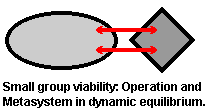
\includegraphics[max width=\textwidth]{2cs2-f1}
\end{center}

Suma had started as a small co-operative in which the Operation and Metasystem were balanced, as described in the study on HWMC. This is illustrated by the diagram shown on the right.

As the numbers grew and the limits to this kind of viability were passed, problems began to emerge.

The structure was still basically the same: the Operation was conceived as a single entity and the once a week all-member meeting was seen as the only Metasystem.

\begin{center}
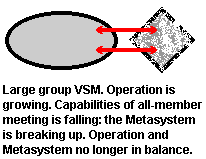
\includegraphics[max width=\textwidth]{2cs2-f2}
\end{center}

The complexity of the Operation was growing explosively in terms of new customers, new products, more services, and more manufacturing, and consequently viability required that the Metasystemic functions had to grow to cope. Some attempts were made to do this (the Finance and Personnel committees) but as the dominant Metasystemic body was the all-member meeting - and as numbers grew beyond 20 this became practically unworkable - the capabilities of the Metasystem were actually decreasing.

In order to deal with this, departments had been set up to deal with the Warehouse, Transport, Manufacturing, Order-picking and so on, but they were still obliged to make all important decisions through the all-member meeting. Thus, they did not have the autonomy they needed to deal with their own problems.

\section*{DIAGNOSIS OF SUMA 1986 (Structure only)}
The diagram opposite shows a VSM with five Operational units (\textbf{O1} to \textbf{O5}). The environment is not shown as the current discussion is limited to the internal structure.

\section*{METASYSTEM}
\begin{center}
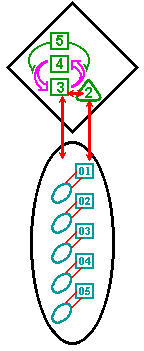
\includegraphics[max width=\textwidth]{2cs2-f3}
\end{center}

\textbf{System 5 (Policy)}

All member meeting. Doesn't work due to number of members.

\textbf{System 4 (Future planning)}

Almost completely absent. Performed by \textit{ad hoc} groups. No 5 year plans. No marketing direction. No formal market research.

System 3 (Synergy)

Some attempts by finance and personnel committees. Hampered by dynamics of all-member meeting. Needs continuous implementation. Some personnel optimisation through the weekly Rota.

\textbf{System 2 (Stability)}

Co-operative ethos and wages policy makes conflict of interests unlikely. Cash flow controlled. Weekly Rota. Fairly robust.

\textbf{System 1 (OPERATION)}

The 5 Operational units illustrated are the Warehouse, Transport, Order Picking, Manufacturing, and Order Taking.

In all cases the problem is the same: the ability to organise the departments effectively is frustrated by the lack of autonomy. The departments, charged with their own internal organisation do not have the freedom they need to work effectively.

\section*{CONCLUSIONS:}
\begin{enumerate}
  \item THE POLICY PROCEDURES NEED TO BE RESTRUCTURED

  \item FUTURE PLANNING AND SYNERGY SYSTEMS NEEDED

  \item STABILITY SYSTEMS NEED TO BE CONSOLIDATED

  \item DEPARTMENTS NEED TO BE MADE AUTONOMOUS WITHIN COHESIVE LIMITS

\end{enumerate}

\section*{THE DOUGHNUT PROPOSALS}
From the above considerations, it became clear that Suma had to rethink itself into autonomous departments. It was equally clear that these departments needed to cohere into a single harmonious organisation. In April 87, four of us produced the Doughnut Proposals which involved local decision making, new functions to articulate the all-Suma Metasystem, and the replacement of the Wednesday meeting with a system of small meetings ("Sectors") which sent delegates to the articulation of System 5 which eventually became known as the "Hub".

The Doughnut proposals involved two VSM fundamentals:

\begin{itemize}
  \item The Operational units must be given as much autonomy (freedom) as possible and the only restrictions involves system cohesion. OR ... you can't give the Operational units complete autonomy as the organisation may fly apart.

  \item Appropriate information gathering and filtration. Whereas the Orwellian view is that information is of use in limiting freedom, the VSM is based upon the principle that information can give an individual the information he needs to organise himself, and thus underwrites individual liberty. The better the information system, the more freedom an individual can have.

\end{itemize}

\section*{IMPLEMENTATION}

\section*{The First 9 Months}
After weeks of debate and lobbying Suma accepted the Doughnut proposals by 25 votes out of the then 29 full members. However, rather than a smooth transition to the structures we proposed, Suma accepted that Things Had To Change and proceeded to try a succession of ideas, some based on the Doughnut proposals, some on the original structures and others on a combination of the two. It was all very unsettling.

One of the problems was that Suma had decided not to drop the old system and go for autonomous departments, but to run the two systems in tandem for a transitional period. While this seemed quite sensible, the old committees refused to relinquish any of their powers and it became clear that they were actually \textbf{preventing} the new structures from becoming effective. It also meant that meetings began to proliferate, as several groups thought it was their job to discuss a particular issue.

After about 6 months of this, the four of us who had produced the original proposals re-convened and produced a further 7 proposals aimed at resolving the situation. Most of these were accepted and implemented immediately; the result still forms the basis of Suma's organisational structure.

\section*{PROPOSALS AND OUTCOMES}
The original proposals were seen as something of a leap in the dark, and most members only accepted them as it was clear \textbf{something} had to be done, and that hierarchical solutions were not acceptable politically.

In the following pages I will take the original proposals (as they were written in 1987), recount what happened in the first few months, and how they developed into our current (1991) structure.

It should be remembered that Suma has been subjected to many other influences over the last five years, and that the Doughnut proposals cannot take the credit for all that has transpired.

The proposals describe the Operational elements as "Segments", the name was later changed to "Sectors".

Similarly the "inter-segment committee" became known as the "Hub".

\section*{PROPOSAL 1: FORMATION OF SEGMENTS}
**

"We propose that Suma formally divides into small groups of around 7 to 10 people.

Each group would work as a close-knit team with responsibility for a particular area of Suma's Operation.

Each group would be given as much autonomy as possible within Suma to deal with its own problems and pursue its own internal development."

**

The Outcome:

Initially very little changed. The theory was that departments could ask for more autonomy as they needed it. During the first year departmental budgets were set up, and thereafter departments had financial autonomy within these limits. And gradually they became more autonomous.

We had originally thought that some small departments might group together into new Operational units - the Segments - but this didn't happen. The original departments stuck to their original form.

Currently most departmental decisions are made internally: all departmental expenditure, and most personnel matters, are dealt with autonomously. It is now recognised that most jobs are fairly specialised and that it would be foolish to have everyone involved in everyone else's business.

Most of the basic conditions for autonomous departments have now become established.

Recent examples are

\begin{enumerate}
  \item The warehouse buys racking and fork trucks from within its budgets.

  \item The office instituted a new system of computerised order taking without reference to the rest of the co-operative.

\end{enumerate}

\section*{PROPOSAL 2: LIMITS TO AUTONOMY}

\section*{PROPOSAL 3: CO-ORDINATION OF SEGMENTS}
**

"Some new functions will be needed to ensure the segments work in a positive way.

We propose a new committee which is formed specifically to ensure the segments work together co-operatively.

This Inter-Segment Committee would consist of one delegate from each segment and would meet once a week to deal with problems between the segments and to suggest ways of improving over-all performance.

We see this committee eventually replacing both the F.C. and the P.C. and forming the basis on which the segments work together."

**

The proposed new meeting, which became known as the Hub, began to meet just as we had intended. However, we had expected it to deal mainly with inter-departmental (nuts and bolts) issues whereas the vast majority of Hub agenda was taken up with all-Suma policy. Initially some internal departmental issues were taken to the Hub, but as the departments were supposed to be autonomous, the Hub referred them back.

\textbf{Essentially the Hub took over from the all-member meeting except for internal departmental issues.}

Currently, the system works as follows:

Once a week everyone who is interested meets in Sectors: groups of about 10 people. They discuss all the issues in the Sector Pack which begins with the minutes from the previous week's meetings, any minutes from other meetings which are relevant, proposals from members and anything else which requires the scrutiny of the whole co-op.

Sector minutes are kept carefully and each meeting sends one delegate to the Hub. The various delegates read the relevant minutes and then make a decision based on the majority view within the co-op. Usually this is straightforward, but some issues are very complex and each Sector may come to a different conclusion. The Hub will usually summarise these views, clarify the lack of consensus and send the issue back for further discussion. Sometimes it becomes clear that a subject requires further thought and as such is referred to a committee. Eventually most Sectors come to similar conclusions and the Hub formalises the decision.

Most decisions are made quickly, a few require two or three trips around the Hub/Sector system, and very occasionally it becomes necessary to call a General Meeting of all members to resolve a particularly difficult issue.

There are two further safeguards on this system:

\begin{itemize}
  \item No Hub decision becomes law until a week after it is made. In this week anyone who may have missed the meeting, can ask for it to be re-discussed in the light of new information.

  \item Any five members can call a General Meeting at any time to discuss an issue they believe has been dealt with badly.

\end{itemize}

These safeguards were introduced to ensure that the Hub did not develop into a managerial elite. In practice they are almost never used: but everyone knows they are there.

\section*{PROPOSAL 4: ACCOUNTABILITY \& COMMUNICATION}
**

"Some way must be found to measure what's going on in each segment so that information is available to co-ordinate and make decisions, and so that segmental Autonomy can be given clear limits.

We propose the use of the system of indices, together with the \textit{Cyberfilter} program to extract important information.

This system puts the responsibility for segmental development on the segments themselves. The information from the system is an immediate representation of what's going on."

**

\textbf{\[Note: The "Cyberfilter" referred to here was a specific implementation of a change-detection system, using the Harrison-Stevens Bayesian forecasting algorithm. This was just one of many potential approaches to detecting incipient instabilities, but one which found favour in mid 1970s VSM applications.\]}

This proposal was without doubt the most radical: we were proposing to move to real-time regulation and to use cybernetic filtration of information in order to generate algedonics. (All of this is described in more detail in Section 6).

There are several aspects to this system:

\begin{itemize}
  \item It provides a complete and current record of all important goings on within each department.

  \item It provides the feedback necessary to enable the members within each department to control their performance.

  \item It gives a structure to Autonomy. Each department was to have an agreed amount of time to solve its problems once an indicator moved outside the acceptable limits.

\end{itemize}

We ran some tests on the systems using the manufacturing department. The indicators measured daily were productivity, machine usage, wastage and happiness. Between them these indicators gave a complete picture of the goings on within this department.

Although the calculation of indicators only took up a few minutes at the end of each day, the system was never formally adopted by the co-op. They were seen to be too difficult to use and at the time there was no interest in making departments accountable.

Over the last five years I have used indicators in the pre-packing department to measure productivity, wastage and out-of-stocks, and still find the system as useful as it seemed originally. However, they are only used within the department - there is still no overall system to ensure the departments are accountable. The only formal system involves the buyers: every week the sales loss through out-of-stocks is measured and plotted as a time series. This is then put in the Sector packs so that everyone knows what is happening. If this indicator began to rise alarmingly, the whole co-operative would know.

There are several other informal performance indicators including daily tonnage, daily sales, the number of lines of orders taken by the sales office, and so on. However the integration of these into formal reporting systems, specific limits to autonomy and overall accountability has never been undertaken.

\section*{PROPOSAL 5: FUTURE PLANNING}
**

"Decision making has already been transformed in the organisational structure proposed so far:

\begin{itemize}
  \item Day by day decisions will be made within close-knit groups and will not clutter up the agenda on a General Meeting.

  \item Co-ordination decisions will be made at weekly meetings of delegates."

\end{itemize}

"This leaves the issue of decisions concerning the outside world as it affects Suma, and long term strategic decisions."

"We propose a new function within Suma to deal with these issues which:

\begin{itemize}
  \item Finds out what's happening in the outside world and its likely effect on Suma. Where appropriate this information can be passed on to the relevant segment.

  \item Considers this information in conjunction with Suma's internal capabilities.

  \item Comes up with FUTURE STRATEGIES about where Suma could be going, marketing, organisation, new products etc.

  \item Thoroughly researches a number of options.

  \item Presents their findings and recommendations to a General Meeting of all members, who make a decision."

\end{itemize}

**

For months, nothing happened whatsoever.

Most of Suma's energies were taken up in dealing with the internal problems and the need for a Futures function was seen as a very low priority.

The issues raised its head again in 1988 after the Hub/Sector system had become established, and this time was pushed hard by the Marketing Department who had recognised the need for a long term marketing strategy, and needed a Business Plan within which to work.

Three members were elected and given the job of researching possible future strategies. A vast number of options were looked at, but nothing actually happened. No proposals were produced.

Currently we have hired consultants to provide us with a 5 year business plan and they have recommended we set up a "Business Plan" group to administer the plan.

However, it would appear that the mechanisms that are being proposed involve analysis of variance and will further strengthen the System 3 (internal control) function. They will not in fact address the need for a System 4 as suggested in these proposals.

\section*{PROPOSAL 6: QUARTERLY GENERAL MEETINGS}
**

"As the general meeting would only be needed to discuss major policy decisions, they would only have to happen every three months.

In exceptional circumstances they may be needed more regularly, and extra-ordinary GMs could be called by the Intra-Segment Committee at any time."

**

As the Hub/Sector system became established it dealt with Policy matters so successfully that General Meetings (of the entire workforce) became almost unnecessary.

Very rarely an issue proves to be too complicated to discuss in separate meetings, and it becomes essential to assemble all the arguments with all the members. This has only happened twice in the last few years.

The new system also allows any 5 members to call an Emergency General Meeting for any reason whatsoever. This has been threatened a few times, but so far it has resulted in the re-discussion of the subject through the Sectors.

Generally it is now accepted that General Meetings are unnecessary except in exceptional circumstances.

\section*{REVIEW OF ORIGINAL DOUGHNUT PROPOSALS}
It's clear that the concept of autonomous departments and the need for a Metasystem to cohere them has worked for Suma.

It's also clear that some of the original details just didn't happen (for example the combination of departments into Segments) and that some of our ideas were re-worked by the co-operative. (For example, the Hub/Sector system was adopted to work almost exclusively with Policy and not with the practicalities of departmental optimisation).

Five years later, it still seems that the basic ideas are sound although the way that we originally interpreted them was far from perfect.

The aspect which we had completely misjudged was the actual implementation. After the acceptance of the proposals, I expected a fairly smooth transition with the support of most of the co-operative.

The reality was that Suma generated a series of excuses for putting off the actual implementation (it's summer so lots of people are on holiday. Now we're getting ready for the Christmas rush ... ) and the actual process had to be pushed very actively.

The details of the period of implementation are not of direct relevance to this case study, although it should be noted that embarking on a programme of radical change in any organisation can be an extremely hazardous occupation.

\section*{FURTHER DEVELOPMENTS}
During the initial implementation, there was a particularly chaotic period during which the Hub self destructed and divested its powers into the Personnel and Finance committees. As these bodies were \textit{a)} designed to deal with a non autonomous Suma, and \textit{b)} able to deal only with specific issues and thus not capable of taking the overall, synoptic view, the situation was unworkable.

In this context, three of the four original Doughnut members met and made a further set of 7 proposals:

**

"If Suma decides to make another attempt at the Doughnut, it's essential to make a much more concerted effort to establish the new system: the old working methods have proved to be more deeply entrenched than we imagined."

"Our proposals are as follows:

**

The crucial elements of the November 87 proposals were accepted and implemented, and still form the basis on which we organise ourselves.

\section*{SUMMARY and ASSESSMENT}
It is clear that the major parts of the System are now in place.

\textbf{System 1: Operation.}

The departments are autonomous within limits set by financial and personnel budgets.

\textbf{System 2: Stability.}

Co-operative working practices continue to keep inter-departmental problems to a minimum. There is now better cash flow control and a recent system of stock control. Stability is further helped by improved co-operative information systems (e.g. the weekly business info).

\textbf{System 3: Optimisation.}

The Finance and Personnel officers \& their committees deal with allocation of resources, and a weekly Rota looks at the best ways of placing personnel. Occasionally committees are set up to deal specifically with optimisation: recently three members were given the task of looking at our job requirements and fitting the best people to each job.

\textbf{System 4: Future Planning.}

The Futures Committee exists although it is presently not functioning in the pro-active way which the VSM sees as fundamental. The eventual outcome is not clear at this point.

\textbf{System 5: Policy}

Suma continues to involve all members in all policy matters on a continuous basis and this has to remain one of the rocks on which the co-operative is organised.

The link between System 1 and System 5 is crucial.

\textbf{The Doughnut proposals began a process of re-organisation which is still in progress. It would be misleading to say that all the proposals were accepted and implemented: it is more accurate to say that we pushed Suma in a particular direction and that the final outcome is the result of the way Suma adapted to that push.}

I view the application generally as a success.

In 1986, the weekly General Meeting had become the most commonly perceived problem. In a recent survey the Hub/Sector system was not even mentioned in the members' list of dissatisfactions. Financially Suma has performed well during the last few years, and seems to be riding out the present recession. The enormous increase in Operational variety over the last three years make it reasonably certain that the pre-VSM structures would not have been able to cope. Had the Autonomy Proposals not been accepted, the only other alternative would have been democratically appointed managers, the introduction of authority-obedience procedures, and consequently the loss of perhaps the most important element of the co-op's success - the self management of most of its members.

It also seems reasonably certain that without VSM theory, the proposals from the Autonomy Group would have been unable to answer many of the criticisms which were levelled at it. The VSM enabled us to present a complete and thorough package, and thus played a crucial role in the development of the co-op.

\section*{Further Enhancements (April 1991)}
There are several areas in which the structure of Suma could still be improved.

\begin{enumerate}
  \item \textbf{Policy}

The Hub/Sector System works wonderfully in keeping everyone involved in policy, However sometimes issues arise which are too complex to discuss in separate meetings, and often a conclusion is avoided. It would seem sensible to make quarterly meetings of all members compulsory in order to resolve these issues, and for everyone to hear from everyone else once in a while.

  \item \textbf{Departmental Optimisation}

The optimisation function has never been formalised. We had originally intended that the "Inter-Segment Group" did the nuts and bolts, how-do-we-work-more-effectively, System 3 stuff, but the Hub developed into a System 5 policy body.

The recent proposal from the business consultants to have a monthly meeting of departmental co-ordinators and to optimise departmental interactions should discharge System 3 effectively, but much depends on the methods they employ for accountability.

  \item \textbf{Performance Indicators}

The performance indicators still look like an extremely efficient means of looking at accountability, of formalising departmental feedback and of putting limits on autonomy. However, they are still so different from usual methods of dealing with organisational information that people are loath to adopt them.

  \item \textbf{Autonomy.}

Departmental autonomy has now become almost complete: the only improvement could be better liaison between the Personnel Officer and Departmental co-ordinators.

Currently some departments are occasionally allocated unsuitable people due to problems with the Rota as a whole.

However, this is a minor quibble - the balance between departmental needs and overall personnel is generally handled well.

  \item \textbf{Futures}

There is still a desperate need for a System 4: someone to keep informed of the markets, external threats and opportunities, and to produce strategies aimed at ensuring Suma can adapt to future eventualities. This must be on a continuous basis, it's clear that System 4 cannot be discharged by an occasional planning meeting.

For an organisation of Suma's size it seems essential to appoint at least one person to do all the System 4 stuff continuously.

\end{enumerate}

\section*{Case Study 3: ONE MONDRAGON CO-OPERATIVE}
This case study is a diagnosis.

I visited \href{https://www.mondragon-corporation.com/en/}{Mondragon} in February 1991 in order to look at the way they handle federations of co-operatives. However, much of what I learned about the organisation of a single enterprise was of such relevance to the use of the VSM, that I felt bound to include it in these case studies.

Many of the conclusions I made concerning Suma have been reached by the Mondragon co-ops, presumably by entirely different routes.

And in many cases they have adopted practical solutions which fit in exactly with some of my more theoretical proposals.

\section*{BACKGROUND}
My visit to Mondragon was primarily to study the way that they manage to get 173 different co-operatives to collaborate. However, the structure of their manufacturing plants has been changing recently, and these changes were of direct relevance to the conclusions I have been coming to through VSM diagnosis.

\href{https://www.mondragon-corporation.com/en/}{Mondragon} are the most successful group of co-operatives that I know, and during the visit I made in February 1991 I was continuously impressed by their commitment to both co-operative ideals and to state-of-the art production techniques. All the factories are full of computer controlled machine tools and robots. They have huge warehouses run entirely by computer. And most of the steel presses and control gear are made by other factories within the Mondragon group.

Some general comments are needed before beginning the description of a single Mondragon co-operative.

\begin{enumerate}
  \item The vocabulary used by the people who escorted us was strikingly similar to that used in the VSM. They think in terms of "autonomy" and use "synergy" regularly. The other word which occurs regularly is "solidarity" which comes as close to Beer's concept of "cohesion" as I can imagine.

  \item To join a Mondragon co-operative every member has to put in the equivalent of about a years salary (around 7,000). 25\% of this goes to the general funds and the individual never sees it again. The other 75\% goes into the individual's account and grows as a percentage of profits is divided amongst the members. The member is not allowed to touch this money until he/she leaves or retires, but interest can be withdrawn.

  \item The co-operatives are organised into Regions and Trade Sectors (again they talk about the need for synergy), and at the end of each financial year the profits of one co-operative are used to offset the losses of another. They say that this is mutual support, and that over the years most co-operatives have had lean patches and have needed financial help.

  \item Distribution of profits is done across a Region or Sector (everyone gets the same) and if the group of co-operatives makes a loss, then money would be withdrawn from individual accounts. So far this hasn't happened.

  \item If jobs are lost in one co-op, the individuals are relocated and to date no-one has had to leave the Mondragon group. While members cannot be guaranteed the same kind of job, so far no-one has been made redundant.

  \item Mondragon has its own social security system which provides health care, sick pay and pensions. If you need a particular operation Mondragon will fly you anywhere in the world and pay all medical expenses.

\end{enumerate}

\section*{ORGANISATION OF ONE MONDRAGON CO-OP}
\begin{center}
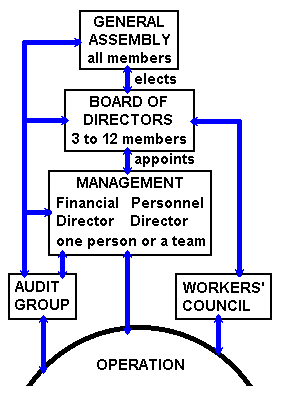
\includegraphics[max width=\textwidth]{p30mond}
\end{center}

\textbf{The General Assembly} meets once or twice a year, involves all members and is concerned with major policy issues, such as membership rules, production targets, budgets and distribution of profits.

Its decisions are binding.

\textbf{The Board of Directors} is elected; members are unpaid and serve for 4 years, meeting once a month. They review and co-ordinate operations, appoint the Management who attend meetings but cannot vote.

It sets Operational policy.

\textbf{The Management} are the executive body of the business, serve for 4 years and have full administrative control.

\textbf{The Audit Group} consists of 3 members elected by the General Assembly who inspect the accounts, sometimes calling in experts. They alert managers of problems (which they are expected to resolve), produce information for the General Assembly, and may alert the Co-op of crisis.

\textbf{The Workers Council} consists of all members. It meets monthly to discuss matters such as wages, conditions and safety. It represents the work force on the Board of Directors.

\textbf{The Operation} covers the basic activities of the system.

\section*{DIAGNOSIS}
At the Metasystemic level, all four VSM functions may be clearly identified.

\textbf{System 5: Policy}

The General Assembly deals with the major policy issues and elects the Board to set Operational policy in its monthly meetings. The Board provides the monitoring function whereby the rest of the Metasystem is seen to operate within policy guidelines.

\textbf{System 4: Long Term Planning}

Long terms plans are drawn up by the Management and sent to the Board for approval. Some debate may follow.

\textbf{System 3: Optimisation}

This is the responsibility of the Management and seems to be taken seriously. They discuss "synergy" between the Operational elements. The Audit group is System 3*, and is a crucial element of System 3 activities. Its job is to provide the information needed to complete System 3's model after the usual information from the business has been obtained. All companies have some sort of audit function - Mondragon seem to have realised the importance of theirs.

\textbf{System 2: Stability}

The Mondragon philosophy provides an extremely effective stabilising system. There are further System 2 bodies like production scheduling and cash flow control. But generally everyone seems to work together well, and conflict of interests get resolved easily.

\textbf{System 1: Operation}

In 1982 the General Assembly decided to change the basic working procedures within the Operation. It was felt that on the shop floor members lacked motivation and that more participation was needed.

They reorganised the production lines into autonomous work groups of about 8 people in which everyone could do all the jobs. Instead of working with a time horizon of 45 seconds , each group had to complete its task in 16 minutes. This gave people time to make a phone call, or have a quick cigarette or whatever.

In the washing machine factory they changed a 300m line with 70 people into 7 lines 30m long, each with 8 people. The change led to a self-organising system, more motivation, and improved productivity and quality.

\textbf{This system of autonomous Operational elements uses performance indicators.} These measure quantity, quality and costs. The daily indicators are measured (e.g. the number produced). Each week they estimate the more subjective measures (e.g. safety, tidiness, autonomy) and give themselves marks out of 10. This number has to be agreed with the foreman who has the final say.

Each work group has responsibility for maintenance, quality, design and so on. At monthly meeting they monitor production targets, discuss problems, arrange training and so on.

\section*{CONCLUSIONS}

\section*{System Design}
Throughout the description of how the Mondragon co-operatives function I found it hard to believe that the system had not been based upon the VSM. In the five years since the Doughnut proposals at Suma I have been attempting to introduce performance indicators, long term planning functions and the like, and almost everything I have been proposing is standard procedure at Mondragon.

Perhaps the only aspect that could be improved is the statistical analysis of the daily information to generate Algedonics automatically. As far as I can tell, they inspect all the information they generate.

\section*{Participation in Policy}
It has always seemed fundamental that all members of a co-operative have the ability to affect policy at all levels and Mondragon seem to adhere to this principle. Within the co-operative all members make policy at yearly meetings, and occasionally at emergency General Assemblies called by a minimum of 10\% of the co-op. During my visit to the Refrigerator factory there were notice boards everywhere full of information on the policy issues which were to be debated at the next General Assembly.

\section*{Representative Management}
They give their elected managers "full administrative authority" although they insist that this can only be maintained if the manager has the trust of the workforce. (He can be removed by an emergency General Assembly.)

It's clear that some Metasystemic functions must be performed without continuous consultation with the work-force (for example long term plans) and at Mondragon they seem to have found a balance between complete authoritarian control and the lack of clear decision making that comes from having to discuss everything with everyone.

The model which was offered to us was that of a busload of people who instruct the driver as to where they want to go, and then leave the details to him. Once he's been instructed, the rest of the people on the bus leave him to operate the brakes, steer and accelerate as he sees fit. The passengers can also direct him to drive more safely, or get another driver if he's no good. But basically it's up to him to drive the bus.

Finally ..

The Mondragon structure seemed to me to be an example of both efficiency and co-operation based firmly upon autonomy and participation. The VSM diagnosis revealed no major flaws, even in the details of how Operational information is gathered.